%! Author = spruhs
%! Date = 25.02.25

% Preamble
\documentclass[11pt]{article}

% Packages
\usepackage[utf8]{inputenc}
\usepackage[T1]{fontenc}
\usepackage[ngerman]{babel}
\usepackage{graphicx}
\usepackage{tcolorbox}
\usepackage{tocloft}
\usepackage{appendix}
\usepackage{csquotes}
\usepackage[
    backend=biber,
    style=alphabetic,
]{biblatex}
\usepackage{color}
\usepackage{listings}
\usepackage{xcolor}
\usepackage{hyperref}
\usepackage[a4paper, left=3cm, right=3cm]{geometry}
\addbibresource{literaturverzeichnis.bib}


% Farben für Syntax-Highlighting definieren
\definecolor{codegreen}{rgb}{0,0.6,0}
\definecolor{codegray}{rgb}{0.5,0.5,0.5}
\definecolor{codepurple}{rgb}{0.58,0,0.82}
\definecolor{backcolour}{rgb}{0.95,0.95,0.92}

% Kotlin-Sprache für listings konfigurieren
\lstdefinelanguage{Kotlin}{
    morekeywords={fun, class, object, val, var, when, if, else, for, while, return, import, package, is, as, null, true, false},
    sensitive=true,
    morecomment=[l]{//},
    morecomment=[s]{/*}{*/},
    morestring=[b]",
}

% Java-Sprache für listings konfigurieren (Java ist bereits vordefiniert, aber hier ein Beispiel für Anpassungen)
\lstdefinelanguage{Java}{
    morekeywords={public, private, protected, class, static, void, if, else, while, for, return, import, package, new},
    sensitive=true,
    morecomment=[l]{//},
    morecomment=[s]{/*}{*/},
    morestring=[b]",
}

\lstset{
    backgroundcolor=\color{backcolour},
    commentstyle=\color{codegreen},
    keywordstyle=\color{codepurple},
    numberstyle=\tiny\color{codegray},
    stringstyle=\color{red},
    basicstyle=\ttfamily\footnotesize,
    breakatwhitespace=false,
    breaklines=true,
    captionpos=b,
    keepspaces=true,
    numbers=left,
    numbersep=5pt,
    showspaces=false,
    showstringspaces=false,
    showtabs=false,
    tabsize=2
}

% Document
\begin{document}

    \begin{titlepage}
        \centering
        {\scshape\LARGE Seminar 1908 Moderne Programmiertechniken und -Methoden -Sommer 2025 \par}
        \vspace{1cm}
        {\huge\bfseries Kotlin statt Java\par}
        \vspace{1.5cm}
        {\scshape\Large Fabian Spruhs\par}
        {\scshape fabian@spruhs.com\par}
        \vspace{2cm}
        {\Large\itshape Studiengang Bachelor Informatik\par}
        \vspace{2cm}


        {\large \today\par}
    \end{titlepage}

    \tableofcontents
    \newpage


    \section{Einleitung}
    Java ist den meisten Entwicklern ein Begriff.
    Es ist eine weit verbreitete Programmiersprache, die seit ihrer Einführung im Jahr 1995 eine zentrale Rolle in der Softwareentwicklung spielt.
    Kotlin ist eine relativ neue Programmiersprache, die 2011 von JetBrains veröffentlicht wurde.
    Sie wurde mit dem Ziel entwickelt, eine moderne und verbesserte Alternative zu Java zu schaffen.
    In diesem Text werden die Unterschiede zwischen Java und Kotlin untersucht.
    Es wird untersucht, inwieweit Kotlin eine geeignete Alternative zu Java darstellt und welche Vorteile Kotlin gegenüber Java bietet.\\
    \\
    Zunächst werden beide Programmiersprachen kurz vorgestellt.
    Anschließend wird auf die Interoperabilität zwischen Java und Kotlin eingegangen.
    Dabei soll gezeigt werden, inwieweit sich Java und Kotlin in einem Projekt kombinieren lassen, bzw. wie bestehende Java-Projekte mit Kotlin weitergeführt werden können.\\
    \\
    Danach werden die unterschiedlichen Features der Sprachen untersucht.
    Zuerst gibt es eine kurze Übersicht über die Features die Kotlin von Java unterscheiden.
    Danach werden die wichtigsten Features genauer erläutert, also die Features die einen tatsächlichen Mehrwert bieten.
    Dabei wird hauptsächlich auf die Unterschiede zwischen Java und Kotlin eingegangen.
    Wie diese Features konkret genutzt werden kann nur am Rande besprochen werden, da dies den Umfang des Textes sprengen würde.\\
    \\
    Zum Schluss gibt es ein Fazit und eine kurze Zusammenfassung der Ergebnisse.
    Die Codebeispiele in diesem Text können auf GitHub unter \url{github.com/FSpruhs/kotlin-statt-java} gefunden werden und können alle, zu Testzwecken, selber ausgeführt werden.\\
    \\
    \section{Kurzvorstellung Java}

    \subsection{Übersicht}
    \begin{itemize}
        \item \textbf{Erscheinungsjahr:} 1995
        \item \textbf{Entwickler:} Sun Microsystems
        \item \textbf{Entwickler ab 2009:} Oracle Corporation
        \item \textbf{Programier paradigmen:} objektorientiert
        \item \textbf{Aktuelle LTS version:} 21
    \end{itemize}

    \subsection{Technischer Hintergrund}
    Java ist eine Programmiersprache, die von Sun Microsystems entwickelt und im Jahr 1995 veröffentlicht wurde.
    Sie zeichnet sich durch ihre Plattformunabhängigkeit, hohe Robustheit und vielseitigen Einsatzmöglichkeiten aus,
    wodurch sie insbesondere in der Industrie und im Unternehmensumfeld eine zentrale Rolle spielt.\\
    \\
    Ein wesentliches Merkmal von Java ist die Art der Code-Ausführung.
    Anstatt direkt in Maschinencode übersetzt zu werden, wird der Quellcode zunächst in Bytecode kompiliert.
    Dieser Bytecode wird anschließend von der Java Virtual Machine (JVM) interpretiert und ausgeführt.
    Durch dieses Konzept ist Java nicht an eine spezifische Prozessorarchitektur oder ein
    bestimmtes Betriebssystem gebunden, was eine hohe Portabilität gewährleistet.
    Diese Plattformunabhängigkeit stellt einen bedeutenden Vorteil dar, den
    viele andere Programmiersprachen im Laufe der Zeit übernommen haben.\\
    \\
    Neben der Plattformunabhängigkeit bietet die JVM zahlreiche zusätzliche
    Funktionen, die zur Stabilität und Sicherheit von Java-Anwendungen beitragen.
    Dazu gehören unter anderem eine automatische Speicherverwaltung
    durch den Garbage Collector, eine starke Typisierung zur Minimierung
    von Laufzeitfehlern sowie eine integrierte Unterstützung für Multithreading,
    die eine effiziente nebenläufige Verarbeitung ermöglicht. \cite[51 - 54]{insel}\\
    \\
    Java basiert konsequent auf dem objektorientierten Programmierparadigma, das die Strukturierung von Software in Klassen und Objekte ermöglicht. \\
    \\
    \subsection{Verbreitung}
    Der TIOBE-Index misst monatlich die Popularität und Verbreitung von Programmiersprachen~\cite{tiobe}.
    Laut diesem Index zählt Java zu den am weitesten verbreiteten Programmiersprachen weltweit.
    Wie in Abbildung~\ref{fig:entwicklung-tiobe} ersichtlich, befand sich Java über fast zwei Jahrzehnte hinweg
    kontinuierlich unter den Top 3 der relevantesten Programmiersprachen.\\
    \\
    In den letzten Jahren hat die Popularität von Java zwar leicht nachgelassen, dennoch bleibt die Sprache weiterhin
    von großer Bedeutung.
    Auch im Februar 2025 belegte Java den dritten Platz im TIOBE-Index (siehe Abbildung~\ref{fig:tiobe-java-2025}).\\
    \\
    Java ist die Basis zahlreicher Anwendungen und wird in vielfältigen Bereichen eingesetzt.
    Darüber hinaus verfügt Java über eine umfangreiche Ökosystemlandschaft mit einer Vielzahl an Bibliotheken, Paketen,Frameworks und Fachliteratur.\\
    \\
    Die weltweite Java-Community ist äußerst aktiv und umfasst eine große Anzahl an erfahrenen Entwicklern, die kontinuierlich zum Wissenstransfer und zur Weiterentwicklung der Sprache beitragen.
    Ein Beispiel für die Größe dieser Infrastruktur ist das Maven-Repository, das über 2.800 Repositories mit mehr als 52 Millionen Java-Paketen enthält~\cite{maven}.\\
    \\
    Diese etablierte und breit aufgestellte Infrastruktur stellt einen weiteren entscheidenden Vorteil von Java dar und
    trägt zu seiner anhaltenden Relevanz in der Softwareentwicklung bei.\\

    \section{Kurzvorstellung kotlin}

    \subsection{Übersicht}
    \begin{itemize}
        \item \textbf{Erscheinungsjahr:} 2011
        \item \textbf{Entwickler:} Jetbrains
        \item \textbf{Programier paradigmen:} objektorientiert, funktional
        \item \textbf{Aktuelle LTS version:} 2.1.0
    \end{itemize}

    \subsection{Technischer Hintergrund}
    Kotlin wurde 2011 von der Firma JetBrains veröffentlicht.
    Ziel der Entwicklung war es, eine verbesserte Alternative zu Java zu schaffen.
    Schon an der Namensgebung kann man die nähe zu Java erkennen.
    Der Name Java bezieht sich auf eine Indonesiche Insel.
    Der Namensgeber von Kotlin ist eine russische Insel vor St. Petersburg.\\
    \\
    Obwohl Java nur etwa 15 Jahre älter als Kotlin ist, stellt dies in der schnelllebigen Welt der Softwareentwicklung eine erhebliche Zeitspanne dar.
    In vielerlei Hinsicht wirkt Java inzwischen veraltet.
    Die Syntax ist vergleichsweise umständlich, und einige moderne Sprachfeatures, die in anderen Programmiersprachen standardmäßig verfügbar sind, fehlen in Java oder
    müssen umständlich über externe Tools nachgerüstet werden.
    Zudem setzt Java ausschließlich auf das objektorientierte Paradigma,
    während moderne Programmiersprachen häufig eine Kombination aus objektorientierter und funktionaler Programmierung unterstützen.\\
    \\
    Bei der Entwicklung von Kotlin hat JetBrains bewusst aus den Designfehlern von Java gelernt.
    Gleichzeitig wurden essenzielle Eigenschaften, die zur Popularität von Java beigetragen haben, beibehalten.\\
    \\
    Kotlin-Code wird ebenfalls in Bytecode kompiliert und kann auf der Java Virtual Machine (JVM) ausgeführt werden.
    Dies bietet den großen Vorteil, dass Kotlin-Programme überall dort lauffähig sind, wo auch Java-Code ausgeführt werden kann.
    Zudem kann Kotlin auf sämtliche vorhandenen Java-Bibliotheken zugreifen und diese nutzen, wodurch nahezu das gesamte Java-Ökosystem zur Verfügung steht.
    Die Interoperabilität zwischen Kotlin und Java geht sogar noch weiter.
    Beide Sprachen lassen sich nahtlos in einem Projekt kombinieren.
    Dadurch können auch bestehende Java-Anwendungen schrittweise mit Kotlin weiterentwickelt werden~\cite[19-20]{kotlin-handbuch}.\\
    \\
    \subsection{Verbreitung}
    Nach dem TIOBE index befindet sich Kotlin im März 2025 nur auf Platz 19 der relevantesten Sprachen, siehe Abbildung~\ref{fig:tiobe-kotlin-2025}.
    Es gibt aber auch gute Nachrichten für Kotlin im Bezug auf die Verbreitung und relevanz.
    Kotlin wurde von Google zu der bevorzugten Sprache für die Android Entwicklung erklärt~\cite{tn3-google}.\\
    \\
    \section{Interoperabilität zwischen Java und Kotlin}

    \subsection{Kotlin in Java integrieren}
    Kotlin und Java lassen sich nahtlos in einem Projekt kombinieren, was zahlreiche Vorteile mit sich bringt.
    Zum einen können in Kotlin geschriebene Klassen und Funktionen problemlos in Java verwendet werden und umgekehrt.
    Zum anderen ermöglicht diese Interoperabilität, bestehende Java-Projekte schrittweise mit Kotlin weiterzuentwickeln oder nach und nach auf Kotlin umzustellen, ohne den vorhandenen Code sofort ersetzen zu müssen.
    Dies ist besonders für Unternehmen mit großen Java-Codebasen relevant, die nicht abrupt auf Kotlin wechseln können~\cite[20]{kotlin-handbuch}.\\
    \\
    Im folgenden Beispiel werden verschiedene Möglichkeiten vorgestellt, wie Kotlin-Code in einer Java-Umgebung ausgeführt werden kann.
    Die zugehörige \texttt{.java}-Datei enthält eine Java-Klasse mit einer \texttt{main}-Methode.
    In dieser Datei wird Kotlin-Code aus einer \texttt{.kt}-Datei importiert und ausgeführt, da Kotlin-Quellcode stets
    in Dateien mit der Endung \texttt{.kt} gespeichert wird.\\
    \\

    \begin{lstlisting}[language=Kotlin, caption={KotlinGreeter.kt}]
package main.java.com.spruhs

class ClassGreeter {
    fun greet() {
        println("Hello from kotlin class method!")
    }
}

class StaticGreeter {
    companion object {

        @JvmStatic
        fun greet() {
            println("Hello from kotlin static method!")
        }
    }
}

object SingletonGreeter {
    fun greet() {
        println("Hello from kotlin singleton method!")
    }
}
    \end{lstlisting}

    \begin{lstlisting}[language=Java, caption={Main.java}]
import main.java.com.spruhs.ClassGreeter;
import main.java.com.spruhs.SingletonGreeter;
import main.java.com.spruhs.StaticGreeter;

public static void main(String[] args) {
    ClassGreeter classGreeter = new ClassGreeter();
    classGreeter.greet();

    StaticGreeter.greet();

    SingletonGreeter.INSTANCE.greet();
}
    \end{lstlisting}

    \begin{tcolorbox}[colback=black!5!white, colframe=black, title=Ausgabe]
        Hello from kotlin class method!\\
        Hello from kotlin static method!\\
        Hello from kotlin singleton method!
    \end{tcolorbox}
    
    \subsection{Java in Kotlin integrieren}
    Auch die umgekehrte Richtung ist problemlos möglich.
    Java-Code lässt sich ohne Weiteres in Kotlin verwenden.
    Dies bietet insbesondere den Vorteil, dass bestehende Java-Bibliotheken und -Frameworks weiterhin genutzt werden können.
    Dies spielt für viele Kotlin-Projekte eine entscheidende Rolle, insbesondere wenn auf etablierte Java-Ökosysteme wie Spring oder Hibernate zurückgegriffen wird.\\
    \\
    Im folgenden Beispiel werden zwei verschiedene Arten gezeigt, wie Java-Klassen in Kotlin eingebunden werden können.
    Einmal über eine Instanzmethode und einmal über eine statische Methode.

    Die Integration von Java in Kotlin ist besonders einfach, da Kotlin die Java-Klassen so behandelt, als wären sie eigene Kotlin-Klassen.
    Statische Methoden und Felder werden in Kotlin über den Klassennamen aufgerufen, Instanzmethoden funktionieren analog wie in Kotlin selbst.
    Damit bietet Kotlin ein hohes Maß an Interoperabilität mit Java, was den Umstieg oder die parallele Nutzung beider Sprachen deutlich vereinfacht.\\
    \\

    \begin{lstlisting}[language=Java, caption={JavaClassMethodGreeter.java}]
package main.kotlin.com.spruhs;

public class JavaClassMethodGreeter {
    public void greet() {
        System.out.println("Hello from java class method!");
    }
}
    \end{lstlisting}

    \begin{lstlisting}[language=Java, caption={JavaStaticGreeter.java}]
package main.kotlin.com.spruhs;

public class JavaStaticGreeter {
    public static void greet() {
        System.out.println("Hello from java static method!");
    }
}

    \end{lstlisting}

    \begin{lstlisting}[language=Kotlin, caption={Main.kt}]
package main.kotlin.com.spruhs

fun main() {
    val javaClassMethodGreeter = JavaClassMethodGreeter()
    javaClassMethodGreeter.greet()

    JavaStaticGreeter.greet()
}
    \end{lstlisting}

    \begin{tcolorbox}[colback=black!5!white, colframe=black, title=Ausgabe]
        Hello from java class method!\\
        Hello from java static method!\\
    \end{tcolorbox}

    \section{Features}

    \subsection{Kurzübersicht}

    In der folgenden Tabelle~\ref{tab:kotlin-java-features} werden zentrale Sprachfeatures aufgeführt, durch die sich Kotlin von Java unterscheidet.
    Anschließend werden einige der wichtigsten Unterschiede genauer erläutert.\\
    \\
    Bei den Features, die Java besitzt, die aber in Kotlin nicht mehr vorhanden sind, lässt sich zwischen vollständig entfallenen Funktionen und solchen unterscheiden, die durch alternative Konzepte ersetzt wurden.\\
    \\
    Ein klassisches Beispiel hierfür sind \texttt{static} Members.
    Kotlin kennt das \texttt{static}-Schlüsselwort nicht.
    Stattdessen bietet Kotlin das Konzept der \texttt{Companion Objects}, um Klassenfunktionen und Klasseneigenschaften zu definieren, die unabhängig von einer konkreten Instanz verfügbar sein sollen.\\
    \\
    Auch das in Java etablierte Konzept der Wildcards (wie \texttt{? extends T} oder \texttt{? super T}) zur Variabilität in generischen Typen wird in Kotlin nicht verwendet.
    An dessen Stelle treten in Kotlin zwei modernere Mechanismen: die Declaration-Site Variance (z.B. \texttt{out T} oder \texttt{in T}) und \texttt{Type Projections}, die eine bessere Lesbarkeit und Typensicherheit ermöglichen.\\
    \\
    Der aus Java bekannte Ternary-Operator (\texttt{condition ? trueExpr : falseExpr}) entfällt in Kotlin vollständig, da \texttt{if}-Anweisungen dort als Ausdrücke gestaltet sind und somit selbst einen Wert zurückgeben können.
    Dadurch lässt sich die gleiche Funktionalität deutlich eleganter realisieren.\\
    \\
    Das Pattern-Matching wird in Kotlin durch die Smart-Casts ersetzt.\\
    \\
    Die mit Java 14 eingeführten \texttt{Records}, die als einfache, immutable Datencontainer dienen, wurden in Kotlin durch die \texttt{data class} ersetzt.
    Diese bieten ähnliche Vorteile, wie automatische Implementierungen von \texttt{equals()}, \texttt{hashCode()} und \texttt{toString()}.\\
    \\
    Checked Exceptions, ein markantes Merkmal der Java-Fehlerbehandlung, existieren in Kotlin nicht mehr.
    Diese Entscheidung wurde bewusst getroffen, da checked exceptions oft als hinderlich für die Lesbarkeit und Wartbarkeit des Codes empfunden werden.
    Fehlerbehandlung in Kotlin erfolgt stattdessen durch unchecked exceptions oder alternative Ansätze wie das Result-Typ-Pattern.
    Hierzu bietet Kotlin den \texttt{Result}-Typ, der eine elegante Möglichkeit zur Handhabung von Erfolgen und Fehlern in einer Funktion bietet.\\
    \\
    Ein weiterer Unterschied liegt in der Sichtbarkeit von Klassen und Mitgliedern.
    Während Java das Schlüsselwort \texttt{package-private} (also ohne Sichtbarkeitsmodifikator) kennt, wurde diese Möglichkeit in Kotlin entfernt.
    In Kotlin gibt es stattdessen die Schlüsselwörter \texttt{public}, \texttt{internal}, \texttt{protected} und \texttt{private}.\\
    \\
    Schließlich ist auch der Umgang mit primitiven Datentypen unterschiedlich: Java unterscheidet streng zwischen primitiven Typen (z.B. int, boolean) und ihren Wrapper-Klassen (Integer, Boolean).
    In Kotlin gibt es diese Trennung nicht auf Sprachebene.
    Hier sind alle Typen Klassen.
    Allerdings sorgt der Kotlin-Compiler dafür, dass im Bytecode bei Bedarf trotzdem die entsprechenden Java-Primitives verwendet werden, um keine Performanceeinbußen zu verursachen.
    \cite{doc-comparison}

    \begin{table}[h!]
        \centering
        \begin{tabular}{|c|c|}
            \hline
            \textbf{Kotlin-Features, die Java nicht hat} & \textbf{Java-Features, die Kotlin nicht hat} \\
            \hline
            \hline
            Lambda expressions & Checked Exceptions \\
            \hline
            Inline functions & Primitive types \\
            \hline
            Extension functions & Wildcard-types \\
            \hline
            Null-safety & Ternary-Operator \\
            \hline
            Default properties & Records \\
            \hline
            Smart casts & Static members \\
            \hline
            Primary constructors & Pattern Matching \\
            \hline
            First-class delegation & package-private visibility modifier \\
            \hline
            Declaration-site variance and Type projections &  \\
            \hline
            Singletons &  \\
            \hline
            Range expressions &  \\
            \hline
            Operator overloading &  \\
            \hline
            Companion objects &  \\
            \hline
            Data classes &  \\
            \hline
            Coroutines &  \\
            \hline
            Top-level functions &  \\
            \hline
            Default arguments &  \\
            \hline
            Named parameters &  \\
            \hline
            Infix functions &  \\
            \hline
            Expect and actual declarations &  \\
            \hline
            Explicit API Mode and better control of API surface &  \\
            \hline
        \end{tabular}
        \caption{Vergleich Kotlin und Java Features}
        \label{tab:kotlin-java-features}
    \end{table}

    \subsection{Null-safety}
    Tony Hoare war 1965 an der Einführung der ersten Null-Referenz in der objektorientierten Sprache ALGOL W beteiligt.
    Im Jahr 2009 bezeichnete er dies rückblickend als den „Milliarden-Dollar-Fehler“~\cite{billion-dollar-mistake}.
    Auch in Java wurde dieser Fehler durch die Einführung von \texttt{null} als Referenzwert übernommen.
    In Java können alle Referenztypen, mit Ausnahme der primitiven Datentypen, den Wert \texttt{null} annehmen.\\
    \\
    Dies führt in der Praxis häufig zu sogenannten \texttt{NullPointerException}, ein weit verbreiteter Laufzeitfehler in Java-Anwendungen.
    Um diese zu vermeiden, müsste man theoretisch jede Referenz vor dem Zugriff auf \texttt{null} prüfen.
    In der Realität wird das jedoch selten konsequent umgesetzt.
    Dies würde auch zu umfangreichem Boilerplate-Code führt, der die Lesbarkeit und Wartbarkeit des Codes stark beeinträchtigen kann.\\
    \\
    Kotlin hat aus diesem Konzeptionsfehler gelernt und verfolgt einen strikt null-sicheren Ansatz.
    In Kotlin sind Referenzen standardmäßig \texttt{non-nullable}.
    Ein Wert kann nur dann \texttt{null} sein, wenn der entsprechende Typ explizit als \texttt{nullable} deklariert wurde.
    Die geschieht durch Anhängen eines Fragezeichens (\texttt{?}) an den Typnamen.
    Der Kotlin-Compiler erzwingt daraufhin eine explizite Überprüfung, wodurch potenzielle \texttt{NullPointerException} bereits zur Compile-Zeit erkannt und vermieden werden können.\\
    \\
    Dieses Sprachfeature trägt erheblich zur Robustheit und Stabilität von Kotlin-Programmen bei, da viele Fehlerquellen bereits zur Entwicklungszeit erkannt werden.
    Darüber hinaus vereinfacht es das Debugging und beschleunigt die Fehlersuche deutlich.
    In Listing~\ref{lst:kotlin-null-safety} wird dieses Prinzip anhand eines einfachen Beispiels verdeutlicht.
    Zwei Variablen des Typs \texttt{String} werden deklariert.
    Eine davon ist \texttt{nullable}, die andere nicht.
    Während der \texttt{nullable} Variablen problemlos \texttt{null} zugewiesen werden kann, führt der gleiche Versuch bei der \texttt{non-nullable} Variablen zu einem Compilerfehler.\\
    \\
    Zusätzlich stellt Kotlin elegante Sprachmittel zur Verfügung, um mit null-Werten umzugehen:

    \begin{itemize}

        \item
            Der Safe-Call-Operator (\texttt{?.}) ermöglicht den Zugriff auf Eigenschaften oder Methoden eines Objekts, ohne zuvor explizit auf null prüfen zu müssen.
            Ist die Referenz \texttt{null}, wird \texttt{null} zurückgegeben, anstatt eine Exception auszulösen.
        \item
            Der Elvis-Operator (\texttt{?:}) erlaubt es, für den Fall eines \texttt{null}-Werts einen Default-Wert zu definieren.
    \end{itemize}

    Diese Mechanismen werden in Listing~\ref{lst:kotlin-user-null-safety} anhand der \texttt{data class KotlinUser} demonstriert.
    Die Funktion \texttt{getUserName} nimmt ein \texttt{nullabel} Objekt entgegen und gibt entweder den enthaltenen Namen oder, falls das Objekt \texttt{null} ist, einen Fallback-Wert zurück.\\
    \\
    Im Vergleich dazu zeigt Listing~\ref{lst:java-user-null-safety} das gleiche Beispiel in Java.
    Dabei wird deutlich, wie viel mehr Boilerplate-Code erforderlich ist, um das gleiche Sicherheitsniveau zu erreichen.\\
    \\

    \begin{lstlisting}[language=Kotlin, caption={KotlinNullSafety.kt}, label={lst:kotlin-null-safety}]
    fun testNullSafety() {
        var nullableVariable: String?
        var nonNullableVariable: String

        nullableVariable = null // Kein Compiler Fehler
        nonNullableVariable = null // Compiler Fehler
    }
    \end{lstlisting}

    \begin{lstlisting}[language=Kotlin, caption={KotlinUser.kt}, label={lst:kotlin-user-null-safety}]
        package main.kotlin.com.spruhs

        fun getUserName(user: KotlinUser?): String {
        return user?.name ?: "Unbekannter Benutzer"
        }

        data class KotlinUser(val name: String)

        fun main() {
        val user1: KotlinUser = KotlinUser("Fabian")
        val user2: KotlinUser? = null

        println(getUserName(user1)) // Ausgabe: Fabian
        println(getUserName(user2)) // Ausgabe: Unbekannter Benutzer
        }
    \end{lstlisting}

    \begin{lstlisting}[language=Java, caption={NullHandlingExample.java}, label={lst:java-user-null-safety}]
    package main.kotlin.com.spruhs;

class JavaUser {
    private String name;

    public JavaUser(String name) {
        this.name = name;
    }

    public String getName() {
        return name;
    }
}

public class NullHandlingExample {
    public static String getUserName(JavaUser user) {
        return (user != null && user.getName() != null) ? user.getName() : "Unbekannter Benutzer";
    }

    public static void main(String[] args) {
        JavaUser user1 = new JavaUser("Fabian");
        JavaUser user2 = null;

        System.out.println(getUserName(user1)); // Ausgabe: Fabian
        System.out.println(getUserName(user2)); // Ausgabe: Unbekannter Benutzer
    }
}
    \end{lstlisting}

    \subsection{Funktionale Programierung}

    Die funktionale Programmierung hat in den letzten Jahren zunehmend an Bedeutung gewonnen.
    Ein wesentlicher Grund dafür liegt in der stagnierenden Entwicklung der CPU-Geschwindigkeit.
    Während in früheren Jahren Leistungssteigerungen hauptsächlich durch höhere Taktfrequenzen erzielt wurden, liegt der Fokus heute verstärkt auf Mehrkernprozessoren.
    Daraus ergibt sich die Notwendigkeit, Programme parallel auszuführen, um die vorhandenen Ressourcen effizient zu nutzen.\\
    \\
    Die funktionale Programmierung eignet sich besonders gut für Parallelisierungskonzepte, da sie auf Zustandslosigkeit und Nebenwirkungsfreiheit basiert.
    Diese Eigenschaften vereinfachen die Ausführung von Code und machen sie zugleich sicherer~\cite[129]{kotlin-patterns}.\\
    \\
    Kotlin wurde von Beginn an mit dem Ziel entwickelt, eine moderne Programmiersprache bereitzustellen, die sowohl objektorientierte als auch funktionale Paradigmen unterstützt.
    Im Gegensatz dazu wurde Java ursprünglich als rein objektorientierte Sprache konzipiert und hat erst mit Version 8 funktionale Sprachmerkmale wie Lambda-Ausdrücke und Streams eingeführt.\\
    \\
    Im Folgenden werden einige der wichtigsten funktionalen Konzepte von Kotlin vorgestellt und mit entsprechenden Merkmalen in Java verglichen.
    Ziel ist es, die Unterschiede sowie die jeweiligen Stärken beider Sprachen im funktionalen Kontext zu verdeutlichen.

    \subsubsection{Higher-Order-Functions}
    Kotlin unterstützt sogenannte Higher-Order Functions.
    Das sind Funktionen, die andere Funktionen als Parameter entgegennehmen oder selbst Funktionen zurückgeben können.
    Funktionen sind in Kotlin sogenannte \textit{First-Class Citizens}, was bedeutet, dass sie wie andere Datentypen behandelt werden können, z.B. indem man sie Variablen zuweist oder als Rückgabewerte verwendet.\\
    \\
    In Java hingegen können Funktionen nicht direkt übergeben werden, da Java ursprünglich keine funktionalen Konzepte vorsah.
    Stattdessen wurde Funktionalität in Methoden gekapselt, die Teil eines Objekts sind.
    Erst mit der Einführung von Lambda-Ausdrücken in Kombination mit functional Interfaces sowie Methoden- und Konstruktorreferenzen in Java 8 wurde eine kompakte Syntax eingeführt, mit der sich Funktionalität auch ohne explizite Klassendefinition umsetzen lässt~\cite[820]{insel}.\\
    \\
    In den folgenden beiden Codebeispielen ist jeweils eine Funktion dargestellt, die zwei Zahlen sowie eine weitere Funktion als Parameter entgegennimmt.
    Diese übergebene Funktion nimmt ebenfalls zwei Zahlen entgegen und gibt eine einzelne Zahl zurück.\\
    \\
    Listing~\ref{lst:kotlin-higher-order-function} zeigt die Kotlin-Variante, während Listing~\ref{lst:java-higher-order-function} die Java-Implementierung darstellt.

    An der Kotlin-Implementierung wird deutlich, dass keine zusätzliche Klasse erforderlich ist.
    Die Funktion kann direkt als Parameter übergeben werden.
    In Java hingegen ist die Übergabe einer Funktion nur über ein funktionales Interface möglich.
    In diesem Fall \texttt{BiFunction}.
    Dieses muss zusätzlich importiert werden.\\
    \\
    Kotlin bietet in diesem Zusammenhang eine deutlich elegantere und direktere Möglichkeit, funktionale Konzepte zu nutzen, da es keine zusätzlichen Konstrukte wie funktionale Interfaces benötigt.\\
    \\

    \begin{lstlisting}[language=Kotlin, caption={HigherOrderKotlin.kt}, label={lst:kotlin-higher-order-function}]
package main.kotlin.com.spruhs

fun operateOnNumbers(a: Int, b: Int, operation: (Int, Int) -> Int): Int {
return operation(a, b)
}

fun main() {
val sum = operateOnNumbers(5, 3) { x, y -> x + y }
println(sum) // Ausgabe 8
}
    \end{lstlisting}

    \begin{lstlisting}[language=Java, caption={HigherOrderJava.java}, label={lst:java-higher-order-function}]
package main.kotlin.com.spruhs;

import java.util.function.BiFunction;

public class HigherOrderJava {

public static int operateOnNumbers(int a, int b, BiFunction<Integer, Integer, Integer> operation) {
return operation.apply(a, b);
}

public static void main(String[] args) {
int sum = operateOnNumbers(5, 3, (x, y) -> x + y);
System.out.println(sum); // Ausgabe 8
}
}
    \end{lstlisting}

    \subsubsection{Inline Functions}
    Kotlin unterstützt sogenannte Inline Functions, mit denen sich der Overhead von Funktionsaufrufen reduzieren lässt.
    Dies ist besonders nützlich in Verbindung mit Higher-Order Functions, da es die Performance verbessert und den generierten Bytecode optimiert.\\
    \\
    Ein vergleichbares Feature in Java sind Lambda-Ausdrücke.
    Diese bieten jedoch nicht den gleichen Grad an Optimierung wie die Inline-Funktionen in Kotlin.
    Bei einer Inline-Funktion wird der Funktionscode direkt an der Aufrufstelle in den Bytecode eingefügt, anstatt zur Laufzeit aufgerufen zu werden.
    Dadurch wird der Overhead vermieden, der bei normalen Funktionsaufrufen entsteht.\\
    \\
    Listing~\ref{lst:kotlin-inline-function} zeigt eine Inline-Funktion in Kotlin.
    Die Funktion \texttt{transformString} nimmt einen \texttt{String} sowie eine Funktion entgegen, die einen \texttt{String} als Parameter akzeptiert und ebenfalls einen \texttt{String} zurückgibt.
    Die übergebene Funktion wird auf den Eingabestring angewendet.
    In diesem Fall wird er in Großbuchstaben umgewandelt.
    Dabei wird bei dem Aufruf der Funktion die übergebene Funktion inline in den Code eingefügt.
    Dies wird durch das Schlüsselwort \texttt{inline} erreicht~\cite{kotlin-inline}.\\
    \\

    \begin{lstlisting}[language=Kotlin, caption={InlineFunction.java}, label={lst:kotlin-inline-function}]
package main.kotlin.com.spruhs

inline fun transformString(input: String, transform: (String) -> String): String {
    return transform(input)
}

fun main() {
    val result = transformString("Hello, World!") { it.uppercase() }
    println(result) // Ausgabe: HELLO, WORLD!
}
    \end{lstlisting}

    \subsection{Threads und Coroutines}

    \subsubsection{Laufzeitverhalten}
    In Java werden Threads verwendet, um parallele Ausführung zu ermöglichen.
    Ein Java Thread ist eine 1 zu 1 Abbildung auf einen Betriebssystem-Thread~\cite[940]{insel}.
    Das bedeutet, dass jeder Java-Thread direkt mit einem Betriebssystem-Thread verknüpft ist.
    Zu jedem Thread gehört dann ein eigener Stack und ein eigener Speicherbereich.
    Threads sind in Java relativ schwergewichtig und benötigen viel Overhead.
    Dadurch kann Java nur eine begrenzte Anzahl von Threads gleichzeitig ausführen.
    Zu viele Threads würden sonst sehr schnell zu einem Mangel an Systemressourcen führen.
    Dieses Problem lässt sich in Java mit Thread-Pools lösen.
    Ein Thread-Pool ist eine Sammlung von Threads, die wiederverwendet werden können, um Aufgaben auszuführen.
    Dabei ist die Anzahl der Threads im Pool begrenzt.
    Wenn ein Thread im Pool blockiert, dann kann dafür kein neuer Thread in den Pool aufgenommen werden.
    Es können erst wieder neue Threads in den Pool aufgenommen werden, wenn ein Thread abgeschlossen ist und der Pool wieder Platz hat.
    Dies führt zu einer nicht optimalen Auslastung der Systemressourcen.\\
    Kotlin bietet eine Alternative zu Threads in Form von Coroutines.
    Coroutines sind leichtgewichtige Threads, die eine einfachere und effizientere Möglichkeit bieten, parallele und asynchrone Programmierung zu implementieren.
    Coroutines sind nicht an einen bestimmten System Thread gebunden und können auf verschiedenen Threads ausgeführt werden.
    Die Verwaltung der Coroutines erfolgt durch den Kotlin-Compiler, der den Overhead von Funktionsaufrufen und Kontextwechseln optimiert.
    Dabei können Coroutines in einem Thread-Pool ausgeführt werden, ohne dass die Anzahl der Threads im Pool begrenzt ist.
    Wenn eine Coroutine blockiert, wird der aktuelle Thread nicht blockiert.
    Dies ermöglicht eine bessere Auslastung der Systemressourcen und eine höhere Effizienz bei der Ausführung von parallelen Aufgaben~\cite[194]{kotlin-patterns}.
    \\
    In Listing~\ref{lst:kotlin-coroutine} wird eine Schleife implementiert die 10.000 durchläuft und dabei einen Zähler um 1 erhöht und dann eine kurze Pause macht und dann nochmal den Zähler um 1 erhöht.
    Diese Schleife ist einmal mit Coroutines und einmal mit Threads implementiert.
    Dabei wird bei den Threads ein Thread-Pool verwendet.
    Die Coroutinen werden ohne einen Thread-Pool gestartet.
    Beide Methoden werden automatisch nach 20 Sekunden abgebrochen, oder sobald die schleife durchgelaufen ist.
    Die Ausführungszeiten der Corotine und der Threads mit verschiedenen Thread-Pools sind in Tabelle~\ref{tab:coroutine-thread-pool} zusammengefasst.
    An der Tabelle ist zu erkennen, dass die Coroutines deutlich schneller sind als die Threads.
    Dies liegt daran, dass die Coroutines nicht an einen bestimmten System-Thread gebunden sind und der Overhead von Funktionsaufrufen und Kontextwechseln optimiert wird.
    Sobald eine Coroutine blockiert, wird der aktuelle Thread nicht blockiert.
    Dadurch können mehrere Coroutines gleichzeitig auf einem Thread ausgeführt werden.
    Der Dispatcher kümmert sich darum, welche Coroutinen gerade blockiert sind und welche bearbeitet werden können.
    Auch kann man an der Tabelle sehen, dass die die Ausführungszeit für mit 2.500 Threads schneller ist als mit 5.000 Threads.
    Eigentlich sollte man davon ausgehen, dass die Ausführungszeit mit mehr Threads auch schneller ist.
    Allerdings steigt mit der Anzahl der Threads auch der Overhead für die Verwaltung der Threads.
    Ab 10000 Threads, also genau der Anzahl der durchläufe, kommt es sogar zu einem OutOfMemoryError.
    An diesem Beispiel lässt sich gut erkennen, dass Coroutines eine leichtgwichtigere Alternative zu den Threads sind.
    Die Messungen wurden auf einem Ubuntu 24.04 System mit 8 GB Arbeitsspeicher und einem AMD Ryzen 5 4500U x 6 Prozessor durchgeführt.\\
    \\

    \begin{lstlisting}[language=Kotlin, caption={Coroutines.kt}, label={lst:kotlin-coroutine}]
package main.kotlin.com.spruhs

import kotlinx.coroutines.*
import java.util.concurrent.CountDownLatch
import java.util.concurrent.Executors
import java.util.concurrent.TimeUnit
import java.util.concurrent.atomic.AtomicInteger

fun coroutineTest() {
    val latch = CountDownLatch(10_000)
    val counter = AtomicInteger()

    val start = System.currentTimeMillis()
    runBlocking {
        for (i in 1..10_000) {
            launch {
                counter.incrementAndGet()
                delay(100)
                counter.incrementAndGet()
                latch.countDown()
            }
        }
    }

    latch.await(20, TimeUnit.SECONDS)

    println("Execution time: ${System.currentTimeMillis() - start} ms, Counter: ${counter.get()/2}")
}

fun threadTest(threadPoolSize: Int) {
    val counter = AtomicInteger()

    val pool = Executors.newFixedThreadPool(threadPoolSize)
    val start = System.currentTimeMillis()
    for (i in 1..10_000) {
        pool.submit {
            counter.incrementAndGet()
            Thread.sleep(100)
            counter.incrementAndGet()
        }
    }

    pool.shutdown()
    pool.awaitTermination(20, TimeUnit.SECONDS)

    println("ThreadPoolSize: $threadPoolSize, execution time: ${System.currentTimeMillis() - start} ms, Counter: ${counter.get()/2}")
}

fun main() {
    coroutineTest()
    listOf(1, 10, 50, 100, 1_000, 2_500, 5_000, 10_000).forEach {
        threadTest(it)
    }
}
    \end{lstlisting}

    \begin{table}[h!]
        \centering
        \begin{tabular}{|c|c|c|c|}
            \hline
             & \textbf{Ausführungszeit} & \textbf{Counter}\\
            \hline
            Coroutines & 396 ms & 10.000   \\
            \hline
            Thread-Pool 1 & 20.045 ms  & 200  \\
            \hline
            Thread-Pool 10 & 20.031 ms  & 1.995  \\
            \hline
            Thread-Pool 50 & 20.056 ms  & 9.975  \\
            \hline
            Thread-Pool 100 & 10.071 ms  & 10.000  \\
            \hline
            Thread-Pool 1.000 & 1.290 ms  & 10.000  \\
            \hline
            Thread-Pool 2.500 & 1.021 ms  & 10.000  \\
            \hline
            Thread-Pool 5.000 & 1.569 ms  & 10.000  \\
            \hline
            Thread-Pool 10.000 & OutOfMemoryError  &   \\
            \hline
        \end{tabular}
        \caption{Ausführungszeiten von Coroutines und Threads}
        \label{tab:coroutine-thread-pool}
    \end{table}

    \subsection{Syntax verbesserungen}
    Kotlin bietet eine Vielzahl von Features die dafür sorgen, dass der Code kürzer ist und das Boilerplate Code reduziert wird.
    Die damit umsetzbare Funktionalitäten lassen sich grundsätzlich auch in Java Code implementieren, erfordern da aber deutlich mehr Boilerplate Code und sind schwieriger zu lesen.
    Damit könnte man diese Features eher als Syntax-Sugar bezeichnen, aber in der Summe bieten diese Features eine deutliche Verbesserung gegenüber Java.
    Die wichtigsten Features werden im Folgenden vorgestellt.

    \subsubsection{Extension Functions}
    Kotlin bietet die Möglichkeit, bestehende Klassen um neue Funktionen zu erweitern, ohne diese Klassen tatsächlich zu ändern.
    Die funktion kann dann wie eine normale Methode aufgerufen werden.
    Mit Extension Functions können nicht nur eigene Klassen erweitert werden, sondern auch Klassen aus externen Bibliotheken.
    In Listing~\ref{lst:kotlin-extension-function} wird eine Extension-Funktion \texttt{double} für die Klasse \texttt{String} implementiert.
    Um eine Extension Function zu implementieren, wird der Typ der Klasse, die erweitert werden soll, vor dem Funktionsnamen angegeben und mit einem Punkt getrennt.
    Diese Funktion verdoppelt den Inhalt des Strings und gibt ihn zurück.
    Mit dem Keyword \texttt{this} kann auf die aktuelle Instanz zugegriffen werden.
    In der \texttt{main}-Methode wird die Funktion zweimal aufgerufen und das Ergebnis ausgegeben.
    In Zeile 8 sieht man sogar, wie schön in in Kotlin die Extension Function direkt von dem String aufgerufen werden kann.
    In Java kann man bestehende Klassen auch erweitern.
    Dazu kann zum Beispiel das Decorator-Pattern verwendet werden oder von der erweiternden Klasse geerbt werden.
    Dies führt aber zu deutlich mehr Boilerplate Code und ist nicht so elegant wie in Kotlin~\cite{kotlin-extensions}.\\
    \\

    \begin{lstlisting}[language=Kotlin, caption={ExtensionFunction.kt}, label={lst:kotlin-extension-function}]
package main.kotlin.com.spruhs

fun String.double(): String {
    return "$this $this"
}

fun main() {
    val name = "Hello World!".double()
    println(name.double()) // Output: Hello World! Hello World! Hello World! Hello World!
}
    \end{lstlisting}

    \subsubsection{Named Parameters, Properties und Primary Constructor}
    Named Parameters und Properties sind zwei Features die oft zusammen verwendet werden.
    Bei Named Parameters handelt es sich um eine Möglichkeit, Parameter in einer Funktion oder einem Konstruktor benennen zu können.
    Dies ermöglicht es, die Parameter in beliebiger Reihenfolge anzugeben und nur die Parameter zu übergeben, die tatsächlich benötigt werden.
    Properties können verwendet werden um einer Klasse Default Attribute hinzuzufügen.
    Dazu kommt noch das Feature des Primary Constructors.
    Der Primary Constructor ist der Konstruktor der Klasse, der direkt in der Klassendeklaration definiert wird.\\
    \\
    In Listing~\ref{lst:kotlin-builder-pattern} wird am Beispiel des Builder Pattern gezeigt, wie Named Parameters, Properties und Primary Constructor zusammen verwendet werden können.
    Bei dem Builder Pattern handelt es sich um eines der klassischen Patterns von der Gang of Four das häufig verwendet wird um Objekte zu erstellen.
    Mit diesem Pattern lässt sich mit nur einem Konstruktor eine Klasse mit einer beliebigen konstellation von Parametern erstellen~\cite{gang-of-four}.
    In der \texttt{class} \texttt{User} werden die Attribute \texttt{firstName}, \texttt{lastName}, \texttt{titles} und \texttt{age} definiert.
    Diese Attribute werden im Primary Constructor der Klasse definiert.
    Diese Attribute sind alle optional und haben Default-Werte.
    In der \texttt{main}-Methode werden zwei Objekt der Klasse \texttt{User} erstellt.
    Dabei hat das erste Objekt alle Attribute und das zweite Objekt nur die Attribute \texttt{firstName} und \texttt{lastName}~\cite[46]{kotlin-patterns}.
    Eine Mögliche implementierung in Java ist in Listing~\ref{lst:java-builder-pattern} zu sehen.
    Diese Implementierung ist deutlich länger und unübersichtlicher als die Kotlin-Implementierung.\\
    \\

    \begin{lstlisting}[language=Kotlin, caption={Builder.kt}, label={lst:kotlin-builder-pattern}]
package main.kotlin.com.spruhs

class User(
    val firstName: String = "",
    val lastName: String = "",
    val titles: List<String> = emptyList(),
    val age: Int? = null,
)

fun main() {
    val user1 = User(
        firstName = "John",
        lastName = "Doe",
        titles = listOf("Mr.", "Dr."),
        age = 30,
    )

    val user2 = User(
        firstName = "Jane",
        lastName = "Smith",
    )
}
    \end{lstlisting}

    \begin{lstlisting}[language=Java, caption={JavaUser.kt}, label={lst:java-builder-pattern}]
        package main.kotlin.com.spruhs;

import java.util.List;

public class JavaUser {
    private String firstName;
    private String lastName;
    private List<String> titles;
    private int age;

    private JavaUser(Builder builder) {
        this.firstName = builder.firstName;
        this.lastName = builder.lastName;
        this.titles = builder.titles;
        this.age = builder.age;
    }

    public static Builder builder() {
        return new Builder();
    }

    public static class Builder {
        private String firstName;
        private String lastName;
        private List<String> titles;
        private int age;

        public Builder firstName(String firstName) {
            this.firstName = firstName;
            return this;
        }

        public Builder lastName(String lastName) {
            this.lastName = lastName;
            return this;
        }

        public Builder titles(List<String> titles) {
            this.titles = titles;
            return this;
        }

        public Builder age(int age) {
            this.age = age;
            return this;
        }

        public JavaUser build() {
            return new JavaUser(this);
        }
    }

    public String getFirstName() { return firstName; }
    public String getLastName() { return lastName; }
    public List<String> getTitles() { return titles; }
    public int getAge() { return age; }
}
    \end{lstlisting}

    \subsubsection{Value Classes}
    Value Objects sind ein wichtiger Bestandteil bei der Implementierung von Domain Driven Design(DDD).
    Ein ziel von von Value Objects im DDD Kontext ist es, die Integrität der Daten zu gewährleisten und sicherzustellen, dass die Objekte in einem konsistenten Zustand sind.
    Weiterhin sollen technische Werte wie Int oder String durch Fachliche Werte ersetzt werden~\cite[219]{red-book}.\\
    \\
    Hierzu können in Kotlin Value Classes verwendet werden.
    Diese sind eine spezielle Art von Klassen, die dazu dienen, einen einzelnen Primitiven Wert zu kapseln und zusätzliche Funktionalität bereitzustellen.
    Zur Laufzeit werden diese Value Classes in den entsprechenden Primitiven Typen umgewandelt.
    Man hat also auf der einen Seite die Laufzeit vorteile von Primitiven Typen und auf der anderen Seite die Typsicherheit und auf der anderen Seite die Möglichkeit, zusätzliche Funktionalität und validierung hinzuzufügen~\cite{kotlin-value-classes}.\\
    \\
    In Listing~\ref{lst:kotlin-value-classes} wird eine Value Class \texttt{NickName} und \texttt{Age} implementiert.
    Dazu wird die Annotation \texttt{@JvmInline} verwendet und das Schlüsselwort value.
    In der Klasse \texttt{Person} werden die Value Classes als Parameter verwendet.
    In der Klassen Deklaration wird beim erstellen der Klasse die der Code in dem \texttt{init} Block ausgeführt.
    Diese werden hier zum validieren der Werte verwendet.
    Eine entsprechende Implementierung in Java ist nicht möglich, da Java keine Value Classes unterstützt.\\
    \\

    \begin{lstlisting}[language=Kotlin, caption={ValueClasses.kt}, label={lst:kotlin-value-classes}]
package main.kotlin.com.spruhs

data class Person(
    val nickName: NickName,
    val age: Age,
)

@JvmInline
value class NickName(val name: String) {
    init {
        require(name.length >= 2 && name.length >= 20) { "NickName must be between 2 and 20 Letters" }
    }
}

@JvmInline
value class Age(val value: Int) {
    init {
        require(value > 0) { "Age must be greater than 0" }
    }
}

fun main() {
    val person = Person(
        nickName = NickName("John"),
        age = Age(30),
    )
}
    \end{lstlisting}

    \subsubsection{Infix Notation}
    Mit der Infix Notation kann man den Aufruf von Extension oder Member Funkionen kürzer schreiben.
    Voraussetzung ist, dass die Funktionen nur einen Parameter, ohne Default Wert, hat.
    In Listing~\ref{lst:kotlin-infix-notation} wird die mit dem Keyword infix die Klasse String um die Funktion \texttt{isLongerThan} erweitert.
    Diese Funktion bekommt einen anderen String übergeben und prüft, ob dieser String kürzer ist als der aktuelle String.
    In Zeile 10 wird die Infix Notation verwendet und diese Funktion aufgerufen, ohne dabei Klammern und Punkt zu benutzten.
    In Zeile 11 passiert das gleiche aber ohne die Infix Notation.
    Beide Aufrufe machen Inhaltlich das gleiche~\cite{kotlin-infix-notation}.\\
    \\

    \begin{lstlisting}[language=Kotlin, caption={InfixNotation.kt}, label={lst:kotlin-infix-notation}]
package main.kotlin.com.spruhs

infix fun String.isLongerThan(other: String): Boolean {
    return this.length > other.length
}

fun main() {
    val hello = "Hello"
    val world = "World!"
    println(hello isLongerThan world) // Output: false
    println(hello.isLongerThan(world)) // Output: false
}
    \end{lstlisting}

    \section{Fazit}

    \printbibliography[
        heading=bibintoc,
        title={Literaturverzeichnis}
    ]
    \appendix
    \section{Anhang}

    \begin{figure}[h]
        \centering
        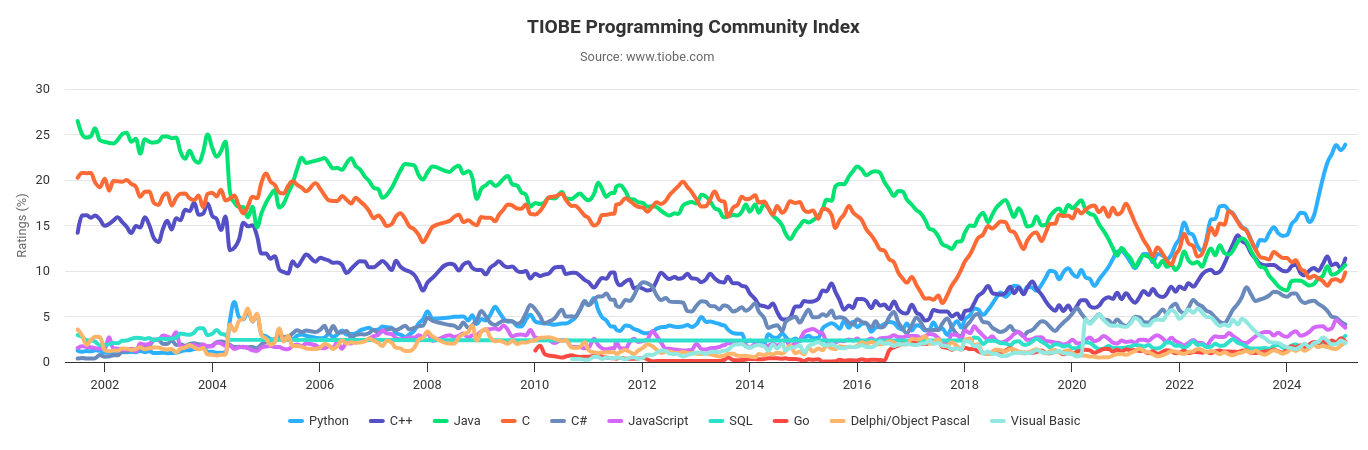
\includegraphics[width=0.8\textwidth]{pictures/Screenshot 2025-02-26 at 19-53-49 TIOBE Index - TIOBE}
        \caption{Entwicklung Tiobe Index 2002 - 2024 vom 26.02.2025 }
        \label{fig:entwicklung-tiobe}
    \end{figure}

    \begin{figure}[h]
        \centering
        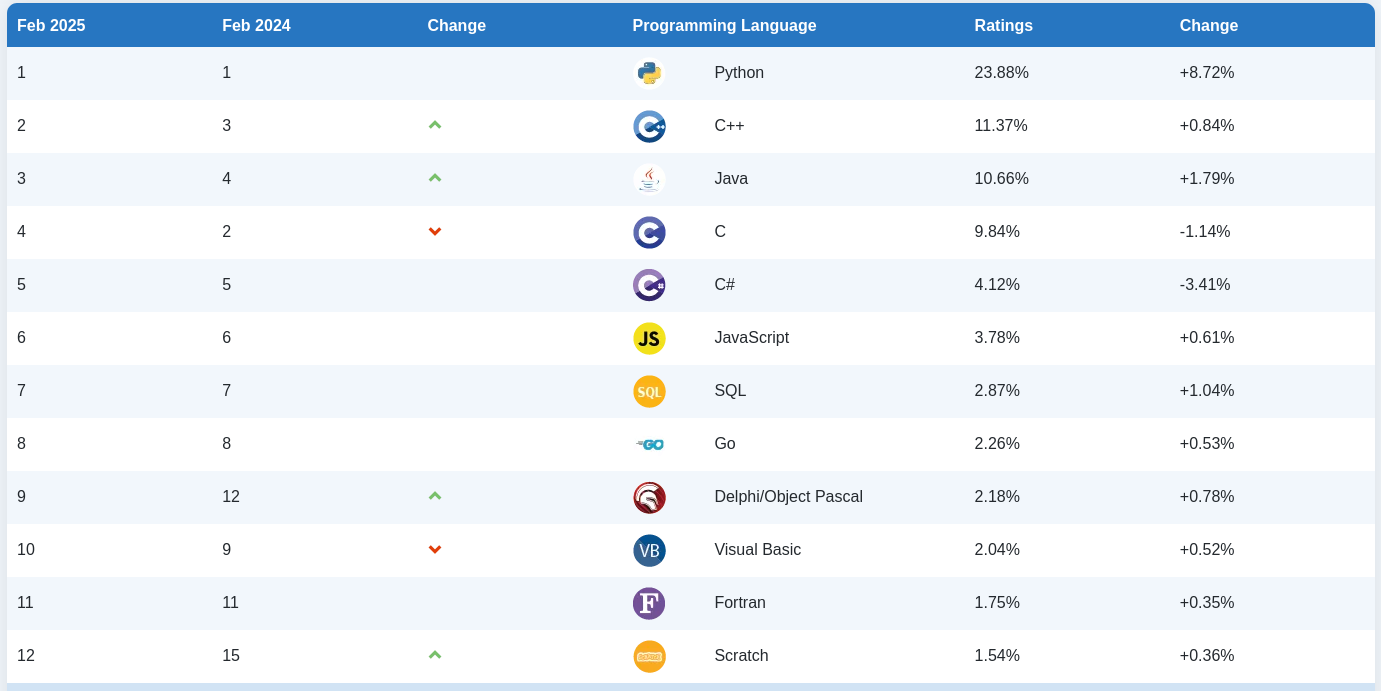
\includegraphics[width=0.8\textwidth]{pictures/Screenshot 2025-02-26 at 19-54-42 TIOBE Index - TIOBE}
        \caption{Tiobe Index Februar 2025 vom 26.02.2025}
        \label{fig:tiobe-java-2025}
    \end{figure}

    \begin{figure}[h]
        \centering
        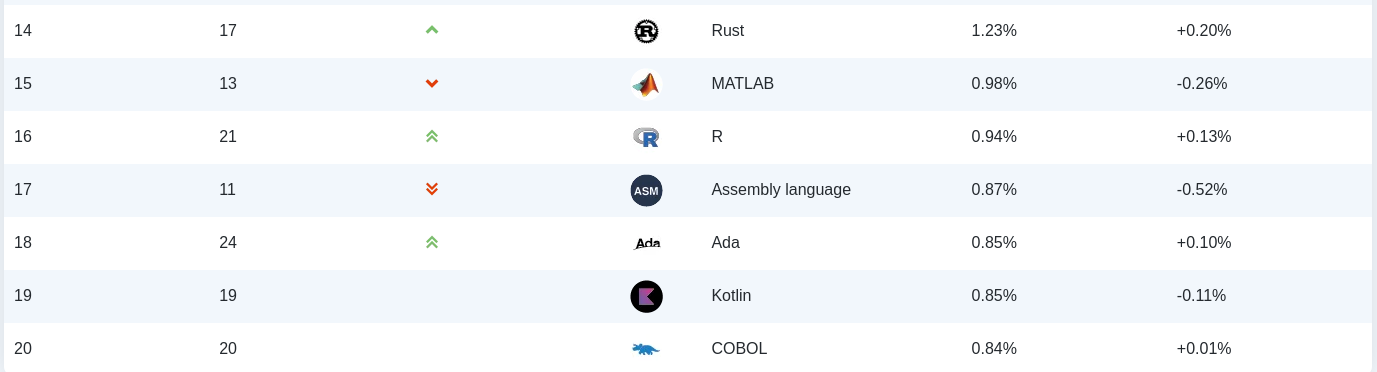
\includegraphics[width=0.8\textwidth]{pictures/Screenshot 2025-03-11 at 22-21-04 TIOBE Index - TIOBE}
        \caption{Tiobe Index März 2025 vom 11.03.2025}
        \label{fig:tiobe-kotlin-2025}
    \end{figure}


\end{document}